\chapter{Planejamento}
\label{planning}

Visando uma jornada livre de imprevistos e dentro do custo e prazo esperados, foi necessário a utilização de um cronograma refinado para auxiliar a equipe. O cronograma citado, foi divido em três macro atividades, organizando o desenvolvimento do projeto desde o seu início até a sua entrega. Como podemos ver na figura \ref{schedule}, as três macro atividades são Iniciação, Elaboração e Construção.

\begin{figure}[htb]
\centering
  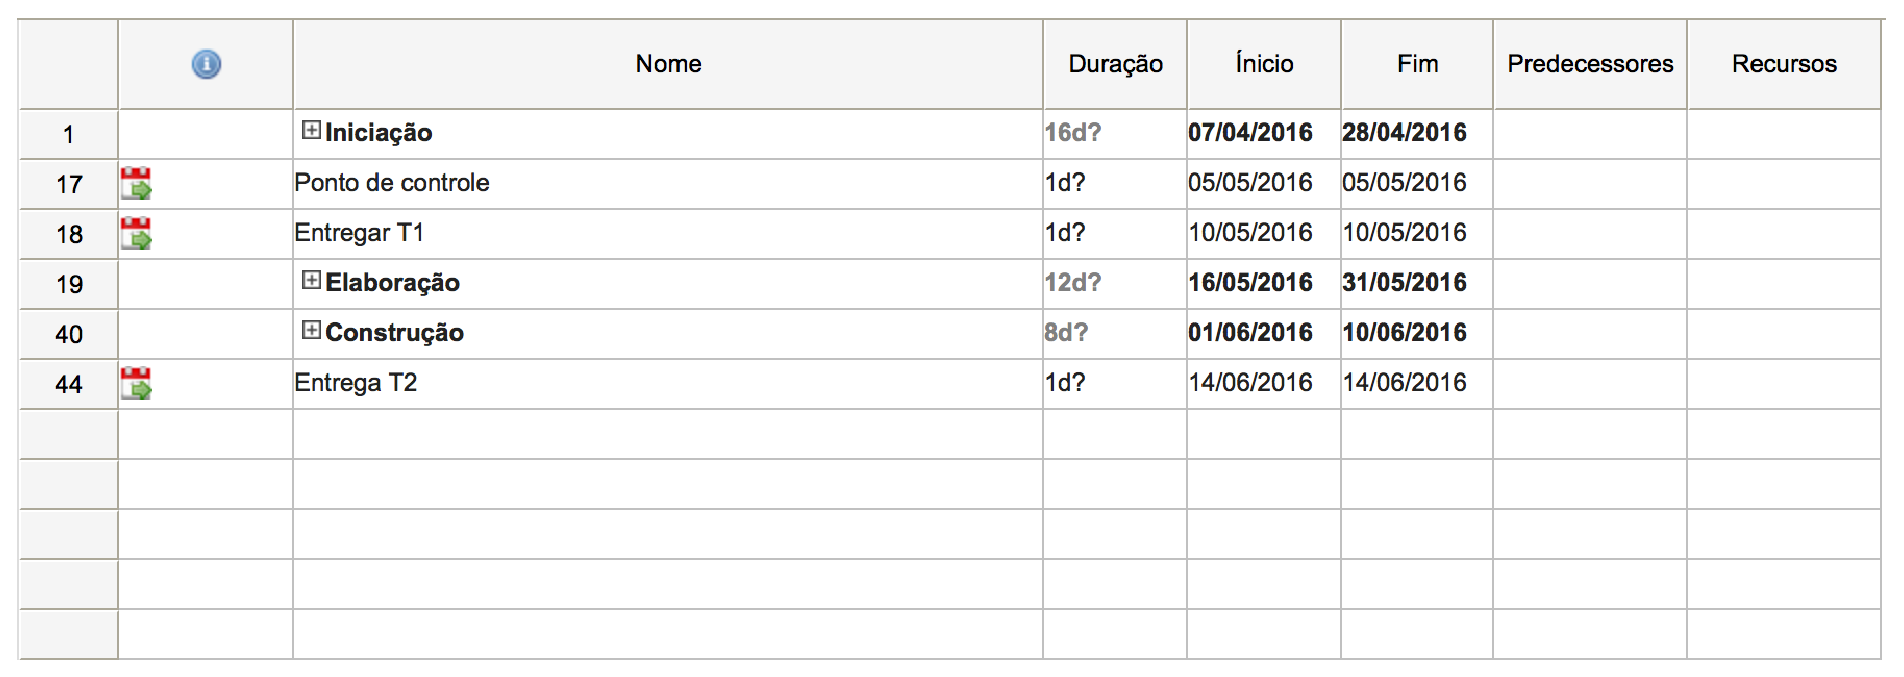
\includegraphics[keepaspectratio=true,scale=0.5]
  {figuras/cronograma_macro.eps}
  \caption{Cronograma dividido por macro atividades}
  \label{schedule}
\end{figure}

\clearpage{}

\section{Iniciação}

Na fase de iniciação, a equipe procurou situar-se em relação ao problema e organizar as atividades, definidas pelo cronograma, para obter uma base para o projeto. Como exemplo dessas atividades está escolher abordagem e definir o processo.

\begin{figure}[htb]
\centering
  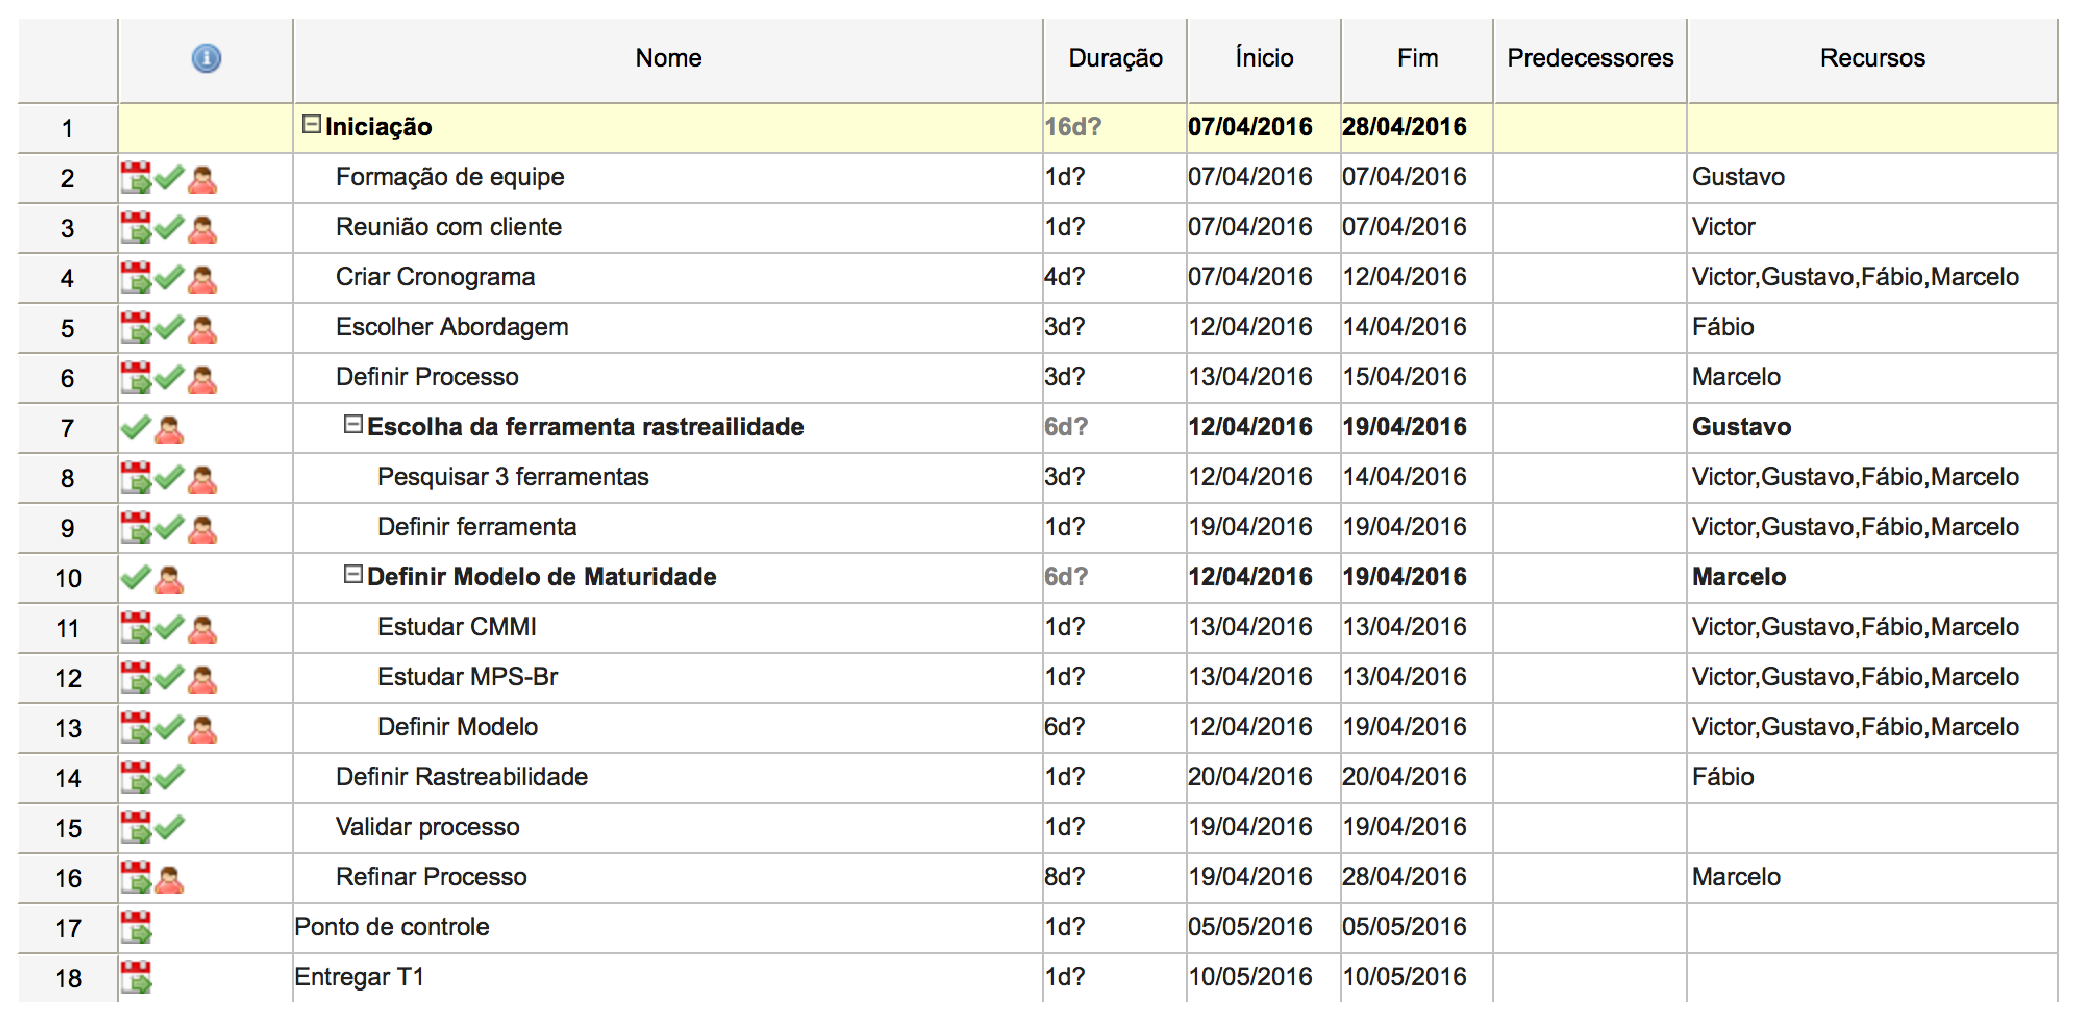
\includegraphics[keepaspectratio=true,scale=0.5]
  {figuras/cronograma_iniciacao.eps}
  \caption{Cronograma na parte de iniciação}
  \label{schedule-init}
\end{figure}

\clearpage{}

\section{Elaboração}

Na fase de elaboração, estão localizadas as atividades que são de fundamental importância para o desenvolvimento da solução proposta. Algumas delas são a elaboração do documento de visão e a priorização de casos de uso.

\begin{figure}[htb]
\centering
  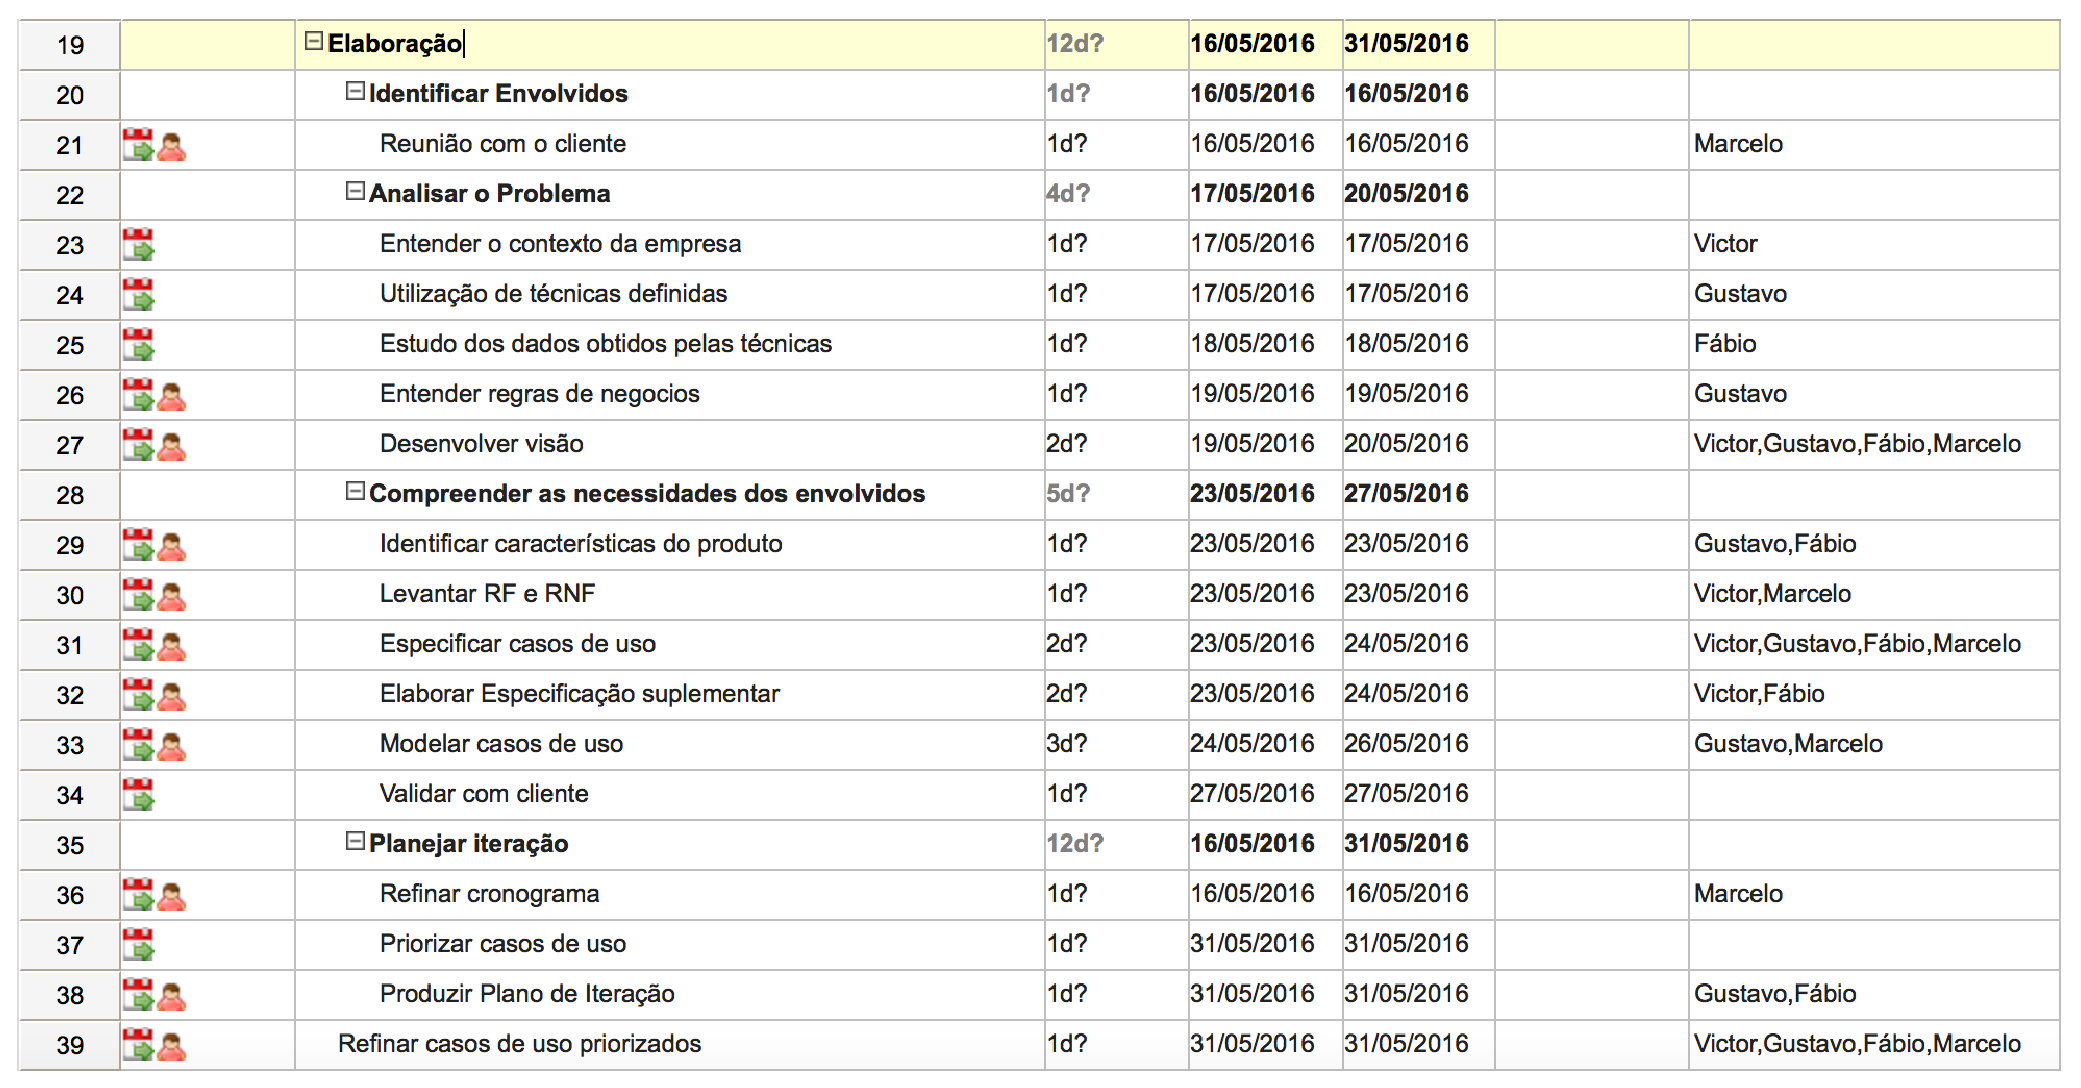
\includegraphics[keepaspectratio=true,scale=0.5]
  {figuras/cronograma_elaboracao.eps}
  \caption{Cronograma na parte de elaboração}
  \label{schedule-elab}
\end{figure}

\clearpage{}

\section{Construção}

Nessa fase, as atividades estão relacionadas ao desenvolvimento do produto. São utilizadas, portanto, as atividades de Engenharia de Requisitos também usadas na fase anterior. O resultado da construção é a entrega parcial do produto através da implementação dos casos de uso priorizados pelo projeto.

\begin{figure}[htb]
\centering
  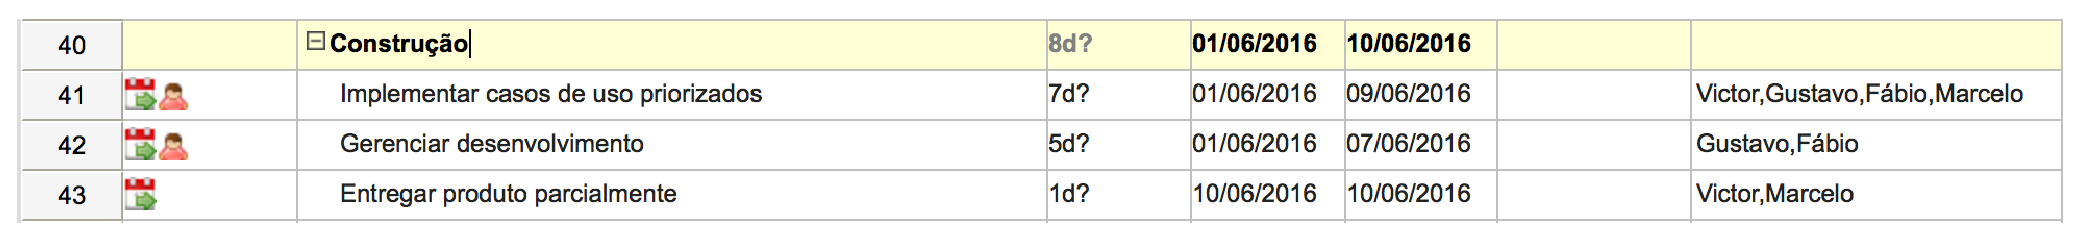
\includegraphics[keepaspectratio=true,scale=0.5]
  {figuras/cronograma_construcao.eps}
  \caption{Cronograma na parte de construção}
  \label{schedule-construct}
\end{figure}

\clearpage{}

